\atspt
    \begin{frame}{\ft{Creating a Data Set from a Book}}
\section{Group 2: Creating a Data Set from a Book}

        \begin{annotatedFigure}{0pt}{19pt}
            {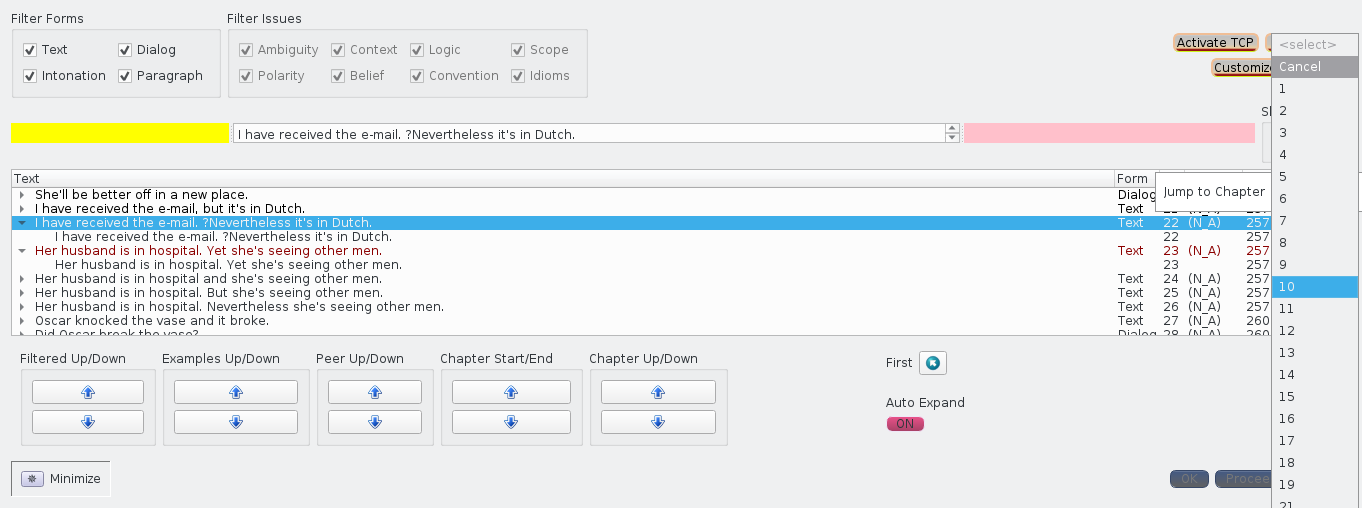
\includegraphics[scale=.86]{texs/chapter.png}}
            
  \node [text width=22.5cm,inner sep=14pt,align=justify,fill=logoCyan!20, %draw=logoBlue, 
  %draw opacity=0.5,
  draw = pink!20!black,
  top color=white,text=black,
  bottom color=pink!40,
  rounded corners=6pt%,
  ]
   at (0.42,1.2){\annfont\textbf{This screenshot shows 
   a linguistics dataset that illustrates several \mbox{advanced} 
   interactive features made possible by the Dataset \mbox{Creator}'s 
   Qt-based front-end technology.  Useful features include context 
   menus \mbox{embedded} with drop-down selections (\circled{1}) and 
   button/checkbox groups for filtered scrolling through 
   a list of samples (\circled{2} and \circled{3}).}};
    
            \annotatedFigureBox{0.93,0.02}{0.985,0.945}{1}{0.985,0.945}%                
            \annotatedFigureBox{0.005,0.82}{0.43,0.98}{2}{0.43,0.82}%
         
            \annotatedFigureBox{0.01,0.1}{0.55,0.334}{3}{0.55,0.334}            
            
      %      \annotatedFigureBox{0.222,0.284}{0.3743,0.4934}{B}{0.3743,0.4934}%tr
      %      \annotatedFigureBox{0.555,0.784}{0.6815,0.874}{C}{0.555,0.784}%bl
      %      \annotatedFigureBox{0.557,0.322}{0.8985,0.5269}{D}{0.8985,0.5269}%tr
  

  
        \end{annotatedFigure}

   %     \caption{Expanded Sample (A)}
    %    \label{fig:teaser}

    \end{frame}

